\documentclass[a4paper]{article}

\usepackage[14pt]{extsizes} % чтобы использовать шрифт размером больше 12
\usepackage{cmap} % для кодировки шрифтов в pdf
\usepackage[T2A]{fontenc} % пакет указывает внутреннюю кодировку в системе LaTeX
\usepackage[utf8]{inputenc} % кодировка  
\usepackage[english, russian]{babel} % пакет для локализации

\usepackage{graphicx} % для вставки картинок
\usepackage{amssymb,amsfonts,amsmath,amsthm} % математические дополнения от АМС
\usepackage{indentfirst} % отделять первую строку раздела абзацным отступом тоже
\usepackage{makecell} % для создания таблиц
\usepackage{multirow} % для продвинутых таблиц
\usepackage{setspace} % для изменения междустрочного интервала
\usepackage{ulem} % подчеркивания
\usepackage{csvsimple} % для импорта csv - таблиц
\usepackage{siunitx,array,booktabs}
\usepackage[tableposition=top]{caption}

\usepackage[left=20mm, top=15mm, right=15mm, bottom=15mm, nohead, footskip=10mm]{geometry} % настройки полей документа

\linespread{1.3} % полуторный интервал
 
\begin{document} % начало документа
 
\section{Математическая модель}

Для решения общей задачи по нахождению деформаций и напряжений в деформируемом теле, занимающем область $G$ с границей $\partial \, G$, необходимо использовать следующие соотношения:

кинематические граничные условия
\begin{equation}
u(x) = u_0, \ x \in \partial \, G_D,
\end{equation}

силовые граничные условия
\begin{equation}
\sigma(u) \cdot n = p(x), \ x \in \partial \, G_N,
\end{equation}

соотношения Коши для тензора полных деформаций
\begin{equation}
\varepsilon(u)=\dfrac{1}{2}(\nabla u + (\nabla u)^T,
\end{equation}

тензор напряжений
\begin{equation}
\sigma(u)=???
\end{equation}

Здесь $u(x)$ - компоненты вектора перемещения, $\partial G_D$ - участок границы, на котором действуют кинематические условия Дирихле, $\partial G_N$ - участок границы, на котором действуют силовые граничные условия Неймана, $p(x)$ - вектор внешней нагрузки. 

Решить данную задачу можно с помощью метода декомпозиции Шварца.

\subsection{Методы Шварца}
Рассмотрим классическую задачу метода Шварца для двух подобластей: имеется сложная область $\Omega$, состоящая из объединения двух простых областей (круга $\Omega_1$ и прямоугольника $\Omega_2$). Рассмотрим уравнение Пуассона, цель которого найти перемещения $u: \Omega \rightarrow \mathbb{R}$ при условии, что
\begin{equation*}
\begin{array}{rl}
-\bigtriangleup \!(u) = f, & u \in \Omega \\
u = 0, & u \in \partial \Omega
\end{array}
\end{equation*}

\begin{figure}[h]
\center{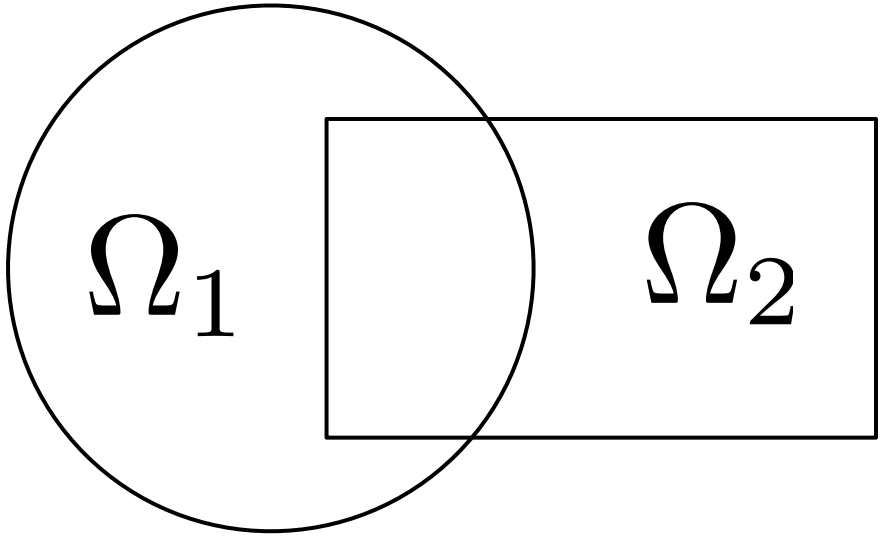
\includegraphics[scale=0.2]{img/simple_domains.png}}
\caption{Сложная область, получившаяся из объединения двух простых областей}
\label{fig:image_01}
\end{figure}

\newpage

Классический метод Шварца это итерационный метод, основанный на решении задач меньшего масштаба в подобластях $\Omega_1$ и $\Omega_2$. Один шаг итерационного процесса обновления результатов $u^n \rightarrow u^{n+1}$:
\begin{equation*}
\begin{array}{rl}
-\bigtriangleup \! (u^{n+1}) = f, & u \in \Omega_1 \\
u^{n+1} = 0, & u \in \partial \Omega_1 \cap \partial \Omega \\
u^{n+1} = u^n, & u \in \partial \Omega_1 \cap \bar{\Omega_2}
\end{array}
\textrm{после чего}
\begin{array}{rl}
-\bigtriangleup \! (u^{n+1}) = f, & u \in \Omega_2 \\
u^{n+1} = 0, & u \in \partial \Omega_2 \cap \partial \Omega \\
u^{n+1} = u^n, & u \in \partial \Omega_2 \cap \bar{\Omega_1}
\end{array}
\end{equation*}

Теперь же рассмотрим случай для произвольной области и произвольного числа подобластей. Вернёмся к нашей первоначальной задаче (ссылка здесь), представим область $G$ в виде объединения конечного числа подобластей $G = \bigcup_{i=1}^{M} G_i$ с конечным числом границ $\partial G_1, \ldots, \partial G_M$, где M - число подобластей. Данные подобласти пересекаются, что требует ввода дополнительных обозначений для границ, возникающих после декомпозиции областей: $\Gamma = \bigcup_{i=1}^{M} \Gamma_i$. 

Выберем начальное приближение для перемещений, удовлетворяющее граничным условиям (ссылка здесь). Алгоритм из классического метода Шварца можно оптимизировать для большего числа подобластей:
\begin{equation*}
\begin{array}{rl}
-\bigtriangleup \! (u^{n+\frac{i}{M}}) = f(x), & x \in G_i \\
\sigma(u^{n+\frac{i}{M}}) \cdot n = p(x), & x \in \partial G_N \cap \partial G_i \\
u^{n+\frac{i}{M}}(x) = 0, & x \in \partial G_D \cap \partial G_i \\ 
u^{n+\frac{i}{M}}(x) = u^{n+\frac{(i - 1)}{M}}(x), & x \in G \setminus ((G_i \setminus \partial G_i) \cap (\partial G_N \cup \partial G_i))
\end{array}
\end{equation*}

Данный алгоритм Шварца называют мультипликативным, он последовательный и решение на каждой подобласти зависит от решения на предыдущей подобласти (или от решения на предыдущей итерации, если речь идёт о первой подобласти для итерации).

Существует также другой вариант метода Шварца, основанный на решении локальных задач для каждой подобласти без зависимости от соседних подобластей:
\begin{equation*}
\begin{array}{rl}
-\bigtriangleup \! (u^{n+\frac{i}{M}}) = f(x), & x \in G_i \\
\sigma(u^{n+\frac{i}{M}}) \cdot n = p(x), & x \in \partial G_N \cap \partial G_i \\
u^{n+\frac{i}{M}}(x) = 0, & x \in \partial G_D \cap \partial G_i \\ 
u^{n+1}(x) = u^{n}(x), & x \in G \setminus ((G_i \setminus \partial G_i) \cap (\partial G_N \cup \partial G_i))
\end{array}
\end{equation*}

Этот метод называется аддитивный метод Шварца. В конце каждой итерации решение вычисляется по формуле 
\begin{equation*}
u^{n+1} = u^{n} + \alpha \sum_{i=1}^{M} (u_i^{n+1} - u^{n}),
\end{equation*}
где коэффициент $\alpha$ - некоторый параметр, от которого зависит скорость сходимости итерационного процесса. 

\newpage

\section{Численная модель}

\newpage

\section{Краткое описание программы}

\newpage

\section{Результаты численных расчётов}

В данном разделе будут приведены расчёты четырёх тестовых задач с использованием четырёх методов. Для каждой из задач для базового случая будут приведены графики распределения напряжений вдоль поверхности, к которой приложено давление, а также графики распределения перемещений на всей расчётной области.

Для методов декомпозиции области расчётные области будут разбиты на заданное количество секторов без перекрытия $\Omega_1, \ldots, \Omega_M$ в зависимости от задачи, где M - число подобластей. Также стоит заметить, что каждая подобласть $\Omega_i$ ($i = 1,\ldots,M$) в зависимости от задачи обладает своими размерными характеристиками. Подобласть $G_i$ соответствует объединению подобласти $\Omega_i$ и дополнительных участков соседних подобластей $\Omega_{i-1}$ и $\Omega_{i+1}$. Размеры этих дополнительных участков зависят от относительного коэффициента перекрытия (отношение размера перекрытия к размеру подобласти $\Omega_i$).

Итерационный процесс для мультипликативного, аддитивного и двухуровневого аддитивного методов продолжается до тех пор, пока не выполнится условие критерия останова $u_{err}$ для перемещений:

\begin{equation*}
u_{err} = \sqrt{\left(\sum_{k = 1}^{N_p} s_k \left(\frac{u_{k}^{m+1} - u_{k}^{m}}{u_{k}^{m+1}} \right)^2\right) / \left(\sum_{k = 1}^{N_{p}} s_k\right)} < \varepsilon_0,
\end{equation*}
где $s_k$ - суммарная площадь элементов сетки, в которые входит $k$-й узел, разделённая на количество узлов в элементе, $N_{elem}$ - количество узлов сетки, $u_{k}^{m+1}$ - решение на текущей итерации, $u_{k}^{m}$ - решение на предыдущей итерации.

Дополнительно для каждой из задач для методов декомпозиции будут приведены таблицы зависимости количества итераций от относительного коэффициента перекрытия.

\newpage

\subsection{Первая тестовая задача}

На рис. \ref{fig:task_01_scheme} представлена расчётная область для первой тестовой задачи - прямоугольник, закреплённый с левой и правой стороны по оси OX и с нижней стороны по оси OY. Сверху действует распределённая нагрузка $p = 50$ МПа. Ширина тела $a = 2$ см, высота тела $b = 1$ см.

\begin{figure}[h]
\center{\includegraphics[scale=0.9]{../results/rectangle/3_fixes/core/area_diagram.png}}
\caption{Схема расчётной области}
\label{fig:task_01_scheme}
\end{figure}

Для решения поставленной задачи примем, что материал тела имеет следующие параметры: модуль Юнга $E = 70$ ГПа, коэффициент Пуассона $\mu = 0.34$. 

Для исследования зависимости сходимости метода от размерности итоговой системы линейных уравнений рассмотрены три расчётные сетки с шагами $h = 0.05$ (количество узлов - 994), $h = 0.025$ (количество узлов - 3812), $h = 0.0125$ (количество узлов - 15006).

Для аддитивного метода Шварца итерационный параметр $\alpha = 0.5$.

\newpage

Для решения задачи методами декомпозиции области расчётная область разбивается по оси OX на заданное количество прямоугольных областей без перекрытия $\Omega_1, \ldots, \Omega_M$. Характерные размеры каждой подобласти: ширина подобласти $a_M = a / M$, высота подобласти совпадает с высотой тела $b_M = b$. На рис. \ref{fig:task_01_decomposition} представлена расчётная область первой тестовой задачи, разбитая на две подобласти.

\begin{figure}[h]
\center{\includegraphics[scale=0.75]{../results/rectangle/3_fixes/core/area_decomposition.png}}
\caption{Схема декомпозиции расчётной области (M = 2)}
\label{fig:task_01_decomposition}
\end{figure}

\newpage

На рис. \ref{fig:task_01_basic_displacement_distribution} приведено распределение перемещений, полученных при решении задачи во всей расчётной области без МДО, на рис. \ref{fig:task_01_basic_pressure_distribution} - распределение напряжений вблизи области приложения давления.

\begin{figure}[h]
\center{\includegraphics[scale=0.75]{../results/rectangle/3_fixes/basic_method/displacement_distribution.png}}
\caption{Распределение перемещений во всей расчётной области}
\label{fig:task_01_basic_displacement_distribution}
\end{figure}

\begin{figure}[h]
\center{\includegraphics[scale=0.2]{../results/rectangle/3_fixes/basic_method/pressure_distribution.png}}
\caption{Распределение напряжений вблизи области приложения давления}
\label{fig:task_01_basic_pressure_distribution}
\end{figure}

\newpage

\subsubsection{Мультипликативный метод Шварца}

В таблице \ref{table:task_01_mult_iters} представлено количество итераций в зависимости от количества подобластей и шага сетки при использовании мультипликативного метода Шварца для первой тестовой задачи (коэффициент захлёста для подобластей равен 0.3). Анализ полученных результатов показал, что:
\begin{itemize}
\item количество итераций не зависит от шага сетки;
\item при увеличении числа подобластей количество итераций увеличивается (при увеличении количества подобластей количество итераций увеличивается примерно в $M^2$ раз);
\end{itemize}

\begin{table}[h]
\caption{Количество итераций в зависимости от количества подобластей и шага сетки}
\csvloop{
	file = ../results/rectangle/3_fixes/schwarz_multiplicative/iters_rectangle.csv,
	head to column names,
	before reading = \centering\sisetup{table-number-alignment=center},
	tabular = {
		@{} |
		c |
		c | 
		c |
		c |
		@{}
	},
	table head = \hline Количество подобластей (M) & \text{h = 0.05} & \text{h = 0.025} & \text{h = 0.0125} \\\hline,
	command = \amnt & \first & \second & \third,
	late after line = \\\hline
}
\label{table:task_01_mult_iters}
\end{table}

\newpage

\subsubsection{Аддитивный метод Шварца}

В таблице \ref{table:task_01_add_iters} представлено количество итераций в зависимости от количества подобластей и шага сетки при использовании аддитивного метода Шварца для первой тестовой задачи (коэффициент захлёста для подобластей равен 0.3). Анализ полученных результатов показал, что:
\begin{itemize}
\item количество итераций несильно зависит от шага сетки;
\item при увеличении числа подобластей количество итераций увеличивается (при увеличении количества подобластей количество итераций увеличивается примерно в $M^2$ раз);
\item количество итераций по сравнению со случаем применения мультипликативного метода Шварца выросло почти в 4 раза;
\end{itemize}

\begin{table}[h]
\caption{Количество итераций в зависимости от количества подобластей и шага сетки}
\csvloop{
	file = ../results/rectangle/3_fixes/schwarz_additive/iters_rectangle.csv,
	head to column names,
	before reading = \centering\sisetup{table-number-alignment=center},
	tabular = {
		@{} |
		c |
		c | 
		c |
		c |
		@{}
	},
	table head = \hline Количество подобластей & \text{h = 0.05} & \text{h = 0.025} & \text{h = 0.0125} \\\hline,
	command = \amnt & \first & \second & \third,
	late after line = \\\hline
}
\label{table:task_01_add_iters}
\end{table}

\newpage

\subsubsection{Двухуровневый аддитивный метод Шварца}
Для двухуровневого аддитивного метода кроме основной сетки в расчётной области зададим грубую сетку, удовлетворяющую условиям включения всех узлов мелкой сетки в элементы грубой сетки и соответствия размеров областей. На рис. \ref{} изображена расчётная область с точками из мелкой сетки и элементами из грубой сетки.

\begin{figure}[h]
\center{\includegraphics[scale=0.9]{../results/rectangle/3_fixes/core/area_diagram.png}}
\caption{Схема расчётной области}
\label{fig:task_01_scheme}
\end{figure}

В таблице \ref{table:task_01_add2_iters} представлено количество итераций в зависимости от количества подобластей и шага сетки при использовании двухуровневого аддитивного метода Шварца для первой тестовой задачи (коэффициент захлёста для подобластей равен 0.3). Анализ полученных результатов показал, что:
\begin{itemize}
\item количество итераций не зависит от шага сетки;
\item при увеличении числа подобластей количество итераций не меняется;
\end{itemize}

\begin{table}[h]
\caption{Количество итераций в зависимости от количества подобластей и шага сетки для двухуровневого аддитивного метода Шварца}
\csvloop{
	file = ../results/rectangle/3_fixes/schwarz_two_level_additive/iters_rectangle.csv,
	head to column names,
	before reading = \centering\sisetup{table-number-alignment=center},
	tabular = {
		@{} |
		c |
		c | 
		c |
		c |
		@{}
	},
	table head = \hline Количество подобластей & \text{h = 0.05} & \text{h = 0.025} & \text{h = 0.0125} \\\hline,
	command = \amnt & \first & \second & \third,
	late after line = \\\hline
}
\label{table:task_01_add2_iters}
\end{table}

В таблице \ref{table:task_01_iters_overlap} рассмотрена зависимость количества итераций от различных вариантов МДО и коэффициента относительного захлёста для случая M = 4 и шага сетки $h = 0.025$. Из таблицы видно, что при росте коэффициента относительного захлёста количество итераций уменьшается.

\begin{table}[h]
\caption{Количество итераций в зависимости от метода декомпозиции области и коэффициента относительного захлёста для случая $M = 4$ и $h = 0.025$}
\csvloop{
	file = ../results/rectangle/3_fixes/core/overlap_rectangle.csv,
	head to column names,
	before reading = \centering\sisetup{table-number-alignment=center},
	tabular = {
		@{} |
		c |
		c |
		c |
		c |
		@{}
	},
	table head = \hline Коэффициент относительного захлёста & 0.2 & 0.3 & 0.4 \\\hline,
	command = \method & \0 & \1 & \2,
	late after line = \\\hline
}
\label{table:task_01_iters_overlap}
\end{table}

\newpage

\subsection{Вторая тестовая задача}

На рис. \ref{fig:task_02_scheme} представлена расчётная область для второй тестовой задачи - прямоугольник, закреплённый с левой стороны по оси OX и с нижней стороны по оси OY. Сверху действует распределённая нагрузка $p = 50$ МПа. Ширина тела $a = 2$ см, высота тела $b = 1$ см.

\begin{figure}[h]
\center{\includegraphics[scale=0.9]{../results/rectangle/2_fixes/core/area_diagram.png}}
\caption{Схема расчётной области}
\label{fig:task_02_scheme}
\end{figure}

Для решения поставленной задачи примем, что материал тела имеет следующие параметры: модуль Юнга $E = 70$ ГПа, коэффициент Пуассона $\mu = 0.34$. 

Для исследования зависимости сходимости метода от размерности итоговой системы линейных уравнений рассмотрены три расчётные сетки с шагами $h = 0.05$ (количество узлов - 994), $h = 0.025$ (количество узлов - 3812), $h = 0.0125$ (количество узлов - 15006).

Для аддитивного метода Шварца итерационный параметр $\alpha = 0.5$.

\newpage

Для решения задачи методами декомпозиции области расчётная область разбивается по оси OX на заданное количество прямоугольных областей без перекрытия $\Omega_1, \ldots, \Omega_M$. Характерные размеры каждой подобласти: ширина подобласти $a_M = a / M$, высота подобласти совпадает с высотой тела $b_M = b$. На рис. \ref{fig:task_02_decomposition} представлена расчётная область вторая тестовой задачи, разбитая на две подобласти.

\begin{figure}[h]
\center{\includegraphics[scale=0.75]{../results/rectangle/2_fixes/core/area_decomposition.png}}
\caption{Схема декомпозиции расчётной области (M = 2)}
\label{fig:task_02_decomposition}
\end{figure}

\newpage

На рис. \ref{fig:task_02_basic_displacement_distribution} приведено распределение перемещений, полученных при решении задачи во всей расчётной области без МДО, на рис. \ref{fig:task_02_basic_pressure_distribution} - распределение напряжений вблизи области приложения давления.

\begin{figure}[h]
\center{\includegraphics[scale=0.75]{../results/rectangle/2_fixes/basic_method/displacement_distribution.png}}
\caption{Распределение перемещений во всей расчётной области}
\label{fig:task_02_basic_displacement_distribution}
\end{figure}

\begin{figure}[h]
\center{\includegraphics[scale=0.2]{../results/rectangle/2_fixes/basic_method/pressure_distribution.png}}
\caption{Распределение напряжений вблизи области приложения давления}
\label{fig:task_02_basic_pressure_distribution}
\end{figure}

\newpage

\subsubsection{Мультипликативный метод Шварца}

В таблице \ref{table:task_02_mult_iters} представлено количество итераций в зависимости от количества подобластей и шага сетки при использовании мультипликативного метода Шварца для второй тестовой задачи (коэффициент захлёста для подобластей равен 0.3). Анализ полученных результатов показал, что:
\begin{itemize}
\item количество итераций не зависит от шага сетки;
\item при увеличении числа подобластей количество итераций увеличивается (при увеличении количества подобластей количество итераций увеличивается примерно в $M^2$ раз);
\end{itemize}

\begin{table}[h]
\caption{Количество итераций в зависимости от количества подобластей и шага сетки}
\csvloop{
	file = ../results/rectangle/2_fixes/schwarz_multiplicative/iters_rectangle.csv,
	head to column names,
	before reading = \centering\sisetup{table-number-alignment=center},
	tabular = {
		@{} |
		c |
		c | 
		c |
		c |
		@{}
	},
	table head = \hline Количество подобластей (M) & \text{h = 0.05} & \text{h = 0.025} & \text{h = 0.0125} \\\hline,
	command = \amnt & \first & \second & \third,
	late after line = \\\hline
}
\label{table:task_02_mult_iters}
\end{table}

\newpage

\subsubsection{Аддитивный метод Шварца}

В таблице \ref{table:task_02_add_iters} представлено количество итераций в зависимости от количества подобластей и шага сетки при использовании аддитивного метода Шварца для второй тестовой задачи (коэффициент захлёста для подобластей равен 0.3). Анализ полученных результатов показал, что:
\begin{itemize}
\item количество итераций несильно зависит от шага сетки;
\item при увеличении числа подобластей количество итераций увеличивается (при увеличении количества подобластей количество итераций увеличивается примерно в $M^2$ раз);
\item количество итераций по сравнению со случаем применения мультипликативного метода Шварца выросло почти в 4 раза;
\end{itemize}

\begin{table}[h]
\caption{Количество итераций в зависимости от количества подобластей и шага сетки}
\csvloop{
	file = ../results/rectangle/3_fixes/schwarz_additive/iters_rectangle.csv,
	head to column names,
	before reading = \centering\sisetup{table-number-alignment=center},
	tabular = {
		@{} |
		c |
		c | 
		c |
		c |
		@{}
	},
	table head = \hline Количество подобластей & \text{h = 0.05} & \text{h = 0.025} & \text{h = 0.0125} \\\hline,
	command = \amnt & \first & \second & \third,
	late after line = \\\hline
}
\label{table:task_02_add_iters}
\end{table}

\newpage

\subsubsection{Двухуровневый аддитивный метод Шварца}

В таблице \ref{table:task_02_add2_iters} представлено количество итераций в зависимости от количества подобластей и шага сетки при использовании двухуровневого аддитивного метода Шварца для первой тестовой задачи (коэффициент захлёста для подобластей равен 0.3). Анализ полученных результатов показал, что:
\begin{itemize}
\item количество итераций не зависит от шага сетки;
\item при увеличении числа подобластей количество итераций не меняется;
\end{itemize}

\begin{table}[h]
\caption{Количество итераций в зависимости от количества подобластей и шага сетки для двухуровневого аддитивного метода Шварца}
\csvloop{
	file = ../results/rectangle/3_fixes/schwarz_two_level_additive/iters_rectangle.csv,
	head to column names,
	before reading = \centering\sisetup{table-number-alignment=center},
	tabular = {
		@{} |
		c |
		c | 
		c |
		c |
		@{}
	},
	table head = \hline Количество подобластей & \text{h = 0.05} & \text{h = 0.025} & \text{h = 0.0125} \\\hline,
	command = \amnt & \first & \second & \third,
	late after line = \\\hline
}
\label{table:task_02_add2_iters}
\end{table}

В таблице \ref{table:task_02_iters_overlap} рассмотрена зависимость количества итераций от различных вариантов МДО и коэффициента относительного захлёста для случая M = 4 и шага сетки $h = 0.025$. Из таблицы видно, что при росте коэффициента относительного захлёста количество итераций уменьшается.

\begin{table}[h]
\caption{Количество итераций в зависимости от метода декомпозиции области и коэффициента относительного захлёста для случая $M = 4$ и $h = 0.025$}
\csvloop{
	file = ../results/rectangle/2_fixes/core/overlap_rectangle.csv,
	head to column names,
	before reading = \centering\sisetup{table-number-alignment=center},
	tabular = {
		@{} |
		c |
		c |
		c |
		c |
		@{}
	},
	table head = \hline Коэффициент относительного захлёста & 0.2 & 0.3 & 0.4 \\\hline,
	command = \method & \0 & \1 & \2,
	late after line = \\\hline
}
\label{table:task_02_iters_overlap}
\end{table}

\newpage

\subsection{Третья тестовая задача}

На рис. \ref{fig:task_03_scheme} представлена расчётная область для второй тестовой задачи - сектор поперечного сечения толстостенной трубы, нагруженной внешним давлением $p = 5$ МПа. Внутренний радиус $p_a = 1$ см, внешний радиус $p_b = 2 $ см.

\begin{figure}[h]
\center{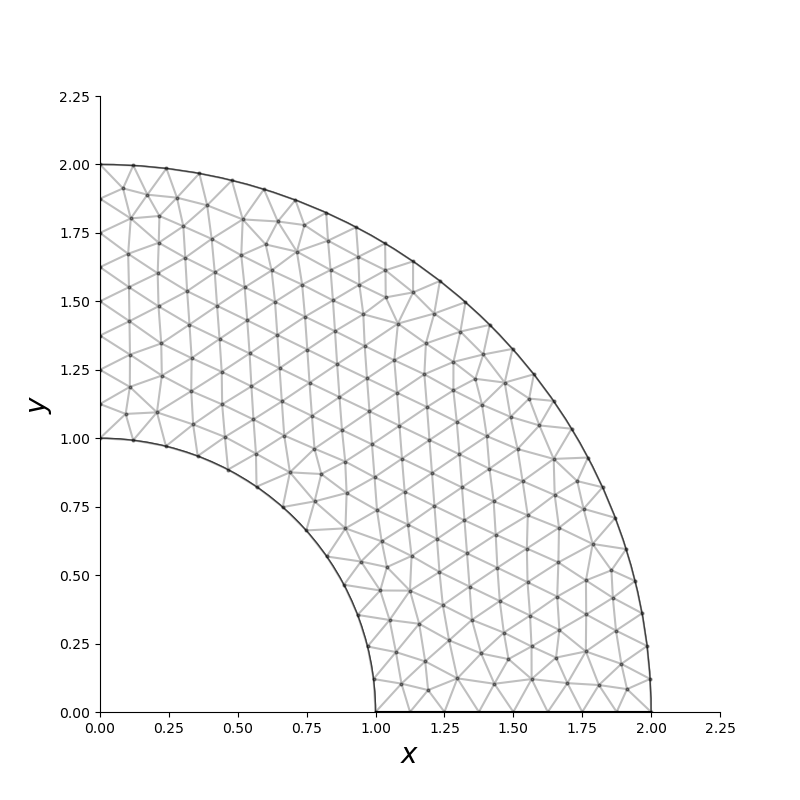
\includegraphics[scale=0.9]{../results/thick_walled_cylinder/pressure_only/core/area_diagram.png}}
\caption{Схема расчётной области третьей тестовой задачи}
\label{fig:task_03_scheme}
\end{figure}

Для решения поставленной задачи примем, что материал тела имеет следующие параметры: модуль Юнга $E = 70$ ГПа, коэффициент Пуассона $\mu = 0.34$. 

Для исследования зависимости сходимости метода от размерности итоговой системы линейных уравнений рассмотрены три расчётные сетки с шагами $h = 0.05$ (количество узлов - 994), $h = 0.025$ (количество узлов - 3812), $h = 0.0125$ (количество узлов - 15006).

Для аддитивного метода Шварца итерационный параметр $\alpha = 0.5$.

\newpage

Для решения задачи методами декомпозиции области расчётная область разбивается на заданное количество секторов без перекрытия $\Omega_1, \ldots, \Omega_M$. 

Характерные размеры каждой подобласти: угол каждого сектора - подобласти $\varphi_M = \pi / (2 \cdot M)$. На рис. \ref{fig:task_03_decomposition} представлена расчётная область третьей тестовой задачи, разбитая на две подобласти.

\begin{figure}[h]
\center{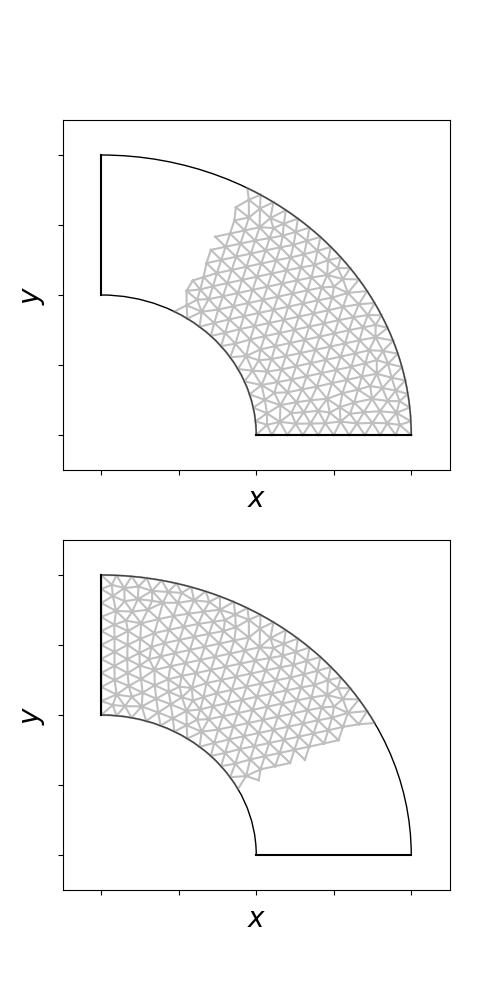
\includegraphics[scale=0.75]{../results/thick_walled_cylinder/pressure_only/core/area_decomposition.png}}
\caption{Схема декомпозиции расчётной области (M = 2)}
\label{fig:task_03_decomposition}
\end{figure}

\newpage

Для третьей тестовой задачи известно аналитическое решение для радиального перемещения и тензора напряженийю. Тогда аналитическое радиальное перемещение считаем по формуле:
\begin{equation*}
u_r = \frac{(1 + \mu) \cdot (1 - 2\mu)}{E}A \cdot r + \frac{(1 + \mu)}{E} \frac{B}{r},
\end{equation*}
где $A = (p_a \cdot r_a^2 - p_b \cdot r_b^2) / (r_b^2 - r_a^2)$, $B = (p_a - p_b) \cdot (r_a r_b)^2 / (r_b^2 - r_a^2)$.

Вычисление аналитического радиального и окружного напряжений производится по формуле:
\begin{equation*}
\sigma_{r, \varphi} = A \mp \frac{B}{r^2}
\end{equation*}

В таблице \ref{table:task_03_basic_errors} представлены относительные ошибки для третьей тестовой задачи, полученные методом без применения МДО для трёх разных шагов сетки, а в таблице \ref{table:task_03_basic_errors_rel} - отношения ошибок. Относительные ошибки вычислялись по формуле:
\begin{equation*}
\sqrt{\left(\sum_{k = 1}^{N_{elem}} {\left(\frac{\sigma_k^{ex} - \sigma_k^{num}}{\sigma_k^{ex}}\right)^2}\right) / \left(\sum_{k=1}^{N_{elem}} {s_k}\right)},
\end{equation*}

где $\sigma_k^{ex}$ - точное значение рассматриваемой компоненты тензора напряжений в центре k-ого элемента, $\sigma_k^{num}$ - полученное численное значение аналогичной величины, $s_k$ - площадь k-го элемента сетки. 

Из таблицы \ref{table:task_03_basic_errors_rel} видно, что для напряжений наблюдается линейная скорость сходимости численного решения к аналитическому при измельчении сетки, для перемещений - квадратичная.
\begin{table}[h]
\caption{Ошибки численного решения в зависимости от шага сетки}
\csvloop{
	file = ../results/thick_walled_cylinder/pressure_only/basic_method/errors.csv,
	head to column names,
	before reading = \centering\sisetup{table-number-alignment=center},
	tabular = {
		@{} |
		c |
		c | 
		c |
		c |
		@{}
	},
	table head = \hline Шаг сетки & \text{$u_r$} & \text{$\sigma_r$} & \text{$\sigma_\varphi$} \\\hline,
	command = \step & \ur & \sigmar & \sigmaphi,
	late after line = \\\hline
}
\label{table:task_03_basic_errors}
\end{table}

\begin{table}[h]
\caption{Отношение ошибок численного решения}
\csvloop{
	file = ../results/thick_walled_cylinder/pressure_only/basic_method/errors_rel.csv,
	head to column names,
	before reading = \centering\sisetup{table-number-alignment=center},
	tabular = {
		@{} |
		c |
		c | 
		c |
		c |
		@{}
	},
	table head = \hline Шаг сетки & \text{$u_r$} & \text{$\sigma_r$} & \text{$\sigma_\varphi$} \\\hline,
	command = \step & \ur & \sigmar & \sigmaphi,
	late after line = \\\hline
}
\label{table:task_03_basic_errors_rel}
\end{table}

\newpage

На рис. \ref{fig:task_03_basic_displacement_distribution} приведено распределение перемещений, полученных при решении задачи без методов декомпозиции области, на рис. \ref{fig:task_03_basic_pressure_distribution} - распределение напряжений вблизи области приложения давления.

\begin{figure}[h]
\center{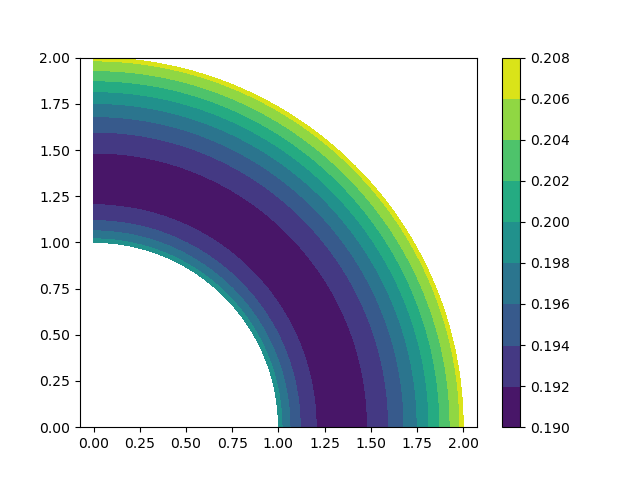
\includegraphics[scale=0.7]{../results/thick_walled_cylinder/pressure_only/basic_method/displacement_distribution.png}}
\caption{Распределение перемещений во всей расчётной области}
\label{fig:task_03_basic_displacement_distribution}
\end{figure}

\begin{figure}[h]
\center{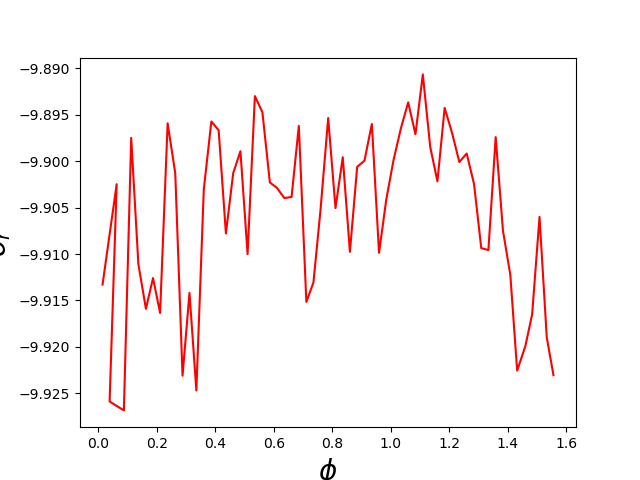
\includegraphics[scale=0.65]{../results/thick_walled_cylinder/pressure_only/basic_method/pressure_distribution.png}}
\caption{Распределение напряжений в расчётной области третьей тестовой задачи}
\label{fig:task_03_basic_pressure_distribution}
\end{figure}

\newpage

\subsubsection{Мультипликативный метод Шварца}

В таблице \ref{table:task_03_mult_iters} представлено количество итераций в зависимости от количества подобластей и шага сетки при использовании мультипликативного метода Шварца в случае фиксированного относительного перекрытия подобластей (данный коэффициент равен 0.3). Анализ полученных результатов показал, что:
\begin{itemize}
\item количество итераций не зависит от шага сетки;
\item при увеличении числа подобластей количество итераций увеличивается;
\end{itemize}

\begin{table}[h]
\caption{Количество итераций в зависимости от количества подобластей и шага сетки для мультипликативного метода Шварца}
\csvloop{
	file = ../results/thick_walled_cylinder/pressure_only/schwarz_multiplicative/iters_thick_walled_cylinder.csv,
	head to column names,
	before reading = \centering\sisetup{table-number-alignment=center},
	tabular = {
		@{} |
		c |
		c | 
		c |
		c |
		@{}
	},
	table head = \hline Количество подобластей & \text{h = 0.05} & \text{h = 0.025} & \text{h = 0.0125} \\\hline,
	command = \amnt & \first & \second & \third,
	late after line = \\\hline
}
\label{table:task_03_mult_iters}
\end{table}

В таблице \ref{table:task_03_mult_iters} представлено количество итераций и ошибки численного решения в зависимости от коэффициента сходимости при шаге сетки $h = 0.0125$ и количестве подобластей $M = 8$ (коэффициент захлёста равен 0.3).


\begin{table}[h]
\caption{Количество итераций и ошибки численного решения в зависимости от коэффициента сходимости}
\csvloop{
	file = ../results/thick_walled_cylinder/pressure_only/schwarz_multiplicative/errors_special.csv,
	head to column names,
	before reading = \centering\sisetup{table-number-alignment=center},
	tabular = {
		@{} |
		c |
		c | 
		c |
		c |
		@{}
	},
	table head = \hline \text{$\varepsilon_0$} & \text{Количество итераций} & $\sigma_r$ & $\sigma_{\varphi}$ \\\hline,
	command = \coefconv & \amnt & \sigmar & \sigmaphi,
	late after line = \\\hline
}
\label{table:task_03_mult_errors_special}
\end{table}

При сравнении таблиц \ref{table:task_03_basic_errors} и \ref{table:task_03_mult_errors_special} можем наблюдать, что ошибки, полученные мультипликативным МДО для $\varepsilon_0 = 10^{-6}$ не отличаются от ошибок, полученных при решении задачи на всей области без применения методов МДО. 

\newpage

\subsubsection{Аддитивный метод Шварца}

В таблице \ref{table:task_03_add_iters} представлено количество итераций в зависимости от количества подобластей и шага сетки при использовании аддитивного метода Шварца в случае фиксированного относительного перекрытия подобластей (данный коэффициент равен 0.3). Анализ полученных результатов показал, что:
\begin{itemize}
\item количество итераций не зависит от шага сетки;
\item при увеличении числа подобластей количество итераций увеличивается;
\end{itemize}

\begin{table}[h]
\caption{Количество итераций в зависимости от количества подобластей и шага сетки для аддитивного метода Шварца}
\csvloop{
	file = ../results/thick_walled_cylinder/pressure_only/schwarz_additive/iters_thick_walled_cylinder.csv,
	head to column names,
	before reading = \centering\sisetup{table-number-alignment=center},
	tabular = {
		@{} |
		c |
		c | 
		c |
		c |
		@{}
	},
	table head = \hline Количество подобластей & \text{h = 0.05} & \text{h = 0.025} & \text{h = 0.0125} \\\hline,
	command = \amnt & \first & \second & \third,
	late after line = \\\hline
}
\label{table:task_03_add_iters}
\end{table}

В таблице \ref{table:task_03_add_iters} представлено количество итераций и ошибки численного решения в зависимости от коэффициента сходимости при шаге сетки $h = 0.0125$ и количестве подобластей $M = 8$ (коэффициент захлёста равен 0.3).

\begin{table}[h]
\caption{Количество итераций и ошибки численного решения в зависимости от коэффициента сходимости}
\csvloop{
	file = ../results/thick_walled_cylinder/pressure_only/schwarz_additive/errors_special.csv,
	head to column names,
	before reading = \centering\sisetup{table-number-alignment=center},
	tabular = {
		@{} |
		c |
		c | 
		c |
		c |
		@{}
	},
	table head = \hline \text{$\varepsilon_0$} & \text{Количество итераций} & $\sigma_r$ & $\sigma_{\varphi}$ \\\hline,
	command = \coefconv & \amnt & \sigmar & \sigmaphi,
	late after line = \\\hline
}
\label{table:task_03_add_errors_special}
\end{table}

При сравнении таблиц \ref{table:task_03_basic_errors} и \ref{table:task_03_add_errors_special} можем наблюдать, что ошибки, полученные мультипликативным МДО для $\varepsilon_0 = 10^{-6}$ не отличаются от ошибок, полученных при решении задачи на всей области без применения методов МДО. 

\newpage

\subsubsection{Двухуровневый аддитивный метод Шварца}

В таблице \ref{table:task_03_add2_iters} представлено количество итераций в зависимости от количества подобластей и шага сетки при использовании двухуровневого аддитивного метода Шварца в случае фиксированного относительного перекрытия подобластей (данный коэффициент равен 0.3). Анализ полученных результатов показал, что:
\begin{itemize}
\item количество итераций не зависит от шага сетки;
\item при увеличении числа подобластей количество итераций не меняется;
\end{itemize}

\begin{table}[h]
\caption{Количество итераций в зависимости от количества подобластей и шага сетки для двухуровневого аддитивного метода Шварца}
\csvloop{
	file = ../results/thick_walled_cylinder/pressure_only/schwarz_two_level_additive/iters_thick_walled_cylinder.csv,
	head to column names,
	before reading = \centering\sisetup{table-number-alignment=center},
	tabular = {
		@{} |
		c |
		c | 
		c |
		c |
		@{}
	},
	table head = \hline Количество подобластей & \text{h = 0.05} & \text{h = 0.025} & \text{h = 0.0125} \\\hline,
	command = \amnt & \first & \second & \third,
	late after line = \\\hline
}
\label{table:task_03_add2_iters}
\end{table}

В таблице \ref{table:task_03_iters_overlap} рассмотрена зависимость количества итераций для различных вариантов методов декомпозиции области от коэффициента относительного перекрытия для случая 4 подобластей и шага сетки $h = 0.025$. Анализ полученных результатов показал, что:
\begin{itemize}
\item при росте коэффициента относительного захлёста количество итераций уменьшается
\end{itemize}

\begin{table}[h]
\caption{Количество итераций в зависимости от метода декомпозиции области и коэффициента относительного захлёста для случая $M = 4$ и $h = 0.025$}
\csvloop{
	file = ../results/thick_walled_cylinder/pressure_only/core/overlap_thick_walled_cylinder.csv,
	head to column names,
	before reading = \centering\sisetup{table-number-alignment=center},
	tabular = {
		@{} |
		c |
		c |
		c |
		c |
		@{}
	},
	table head = \hline Коэффициент относительного захлёста & 0.2 & 0.3 & 0.4 \\\hline,
	command = \method & \0 & \1 & \2,
	late after line = \\\hline
}
\label{table:task_03_iters_overlap}
\end{table}

\newpage

Для улучшения ситуации решения третьей тестовой задачи двухуровневым аддитивным методом можно использовать в качестве грубой сетки сектор поперечного сечения цилиндра. Радиус цилиндра совпадает с внешним радиусом толстостенной трубы.

\begin{figure}[h]
\center{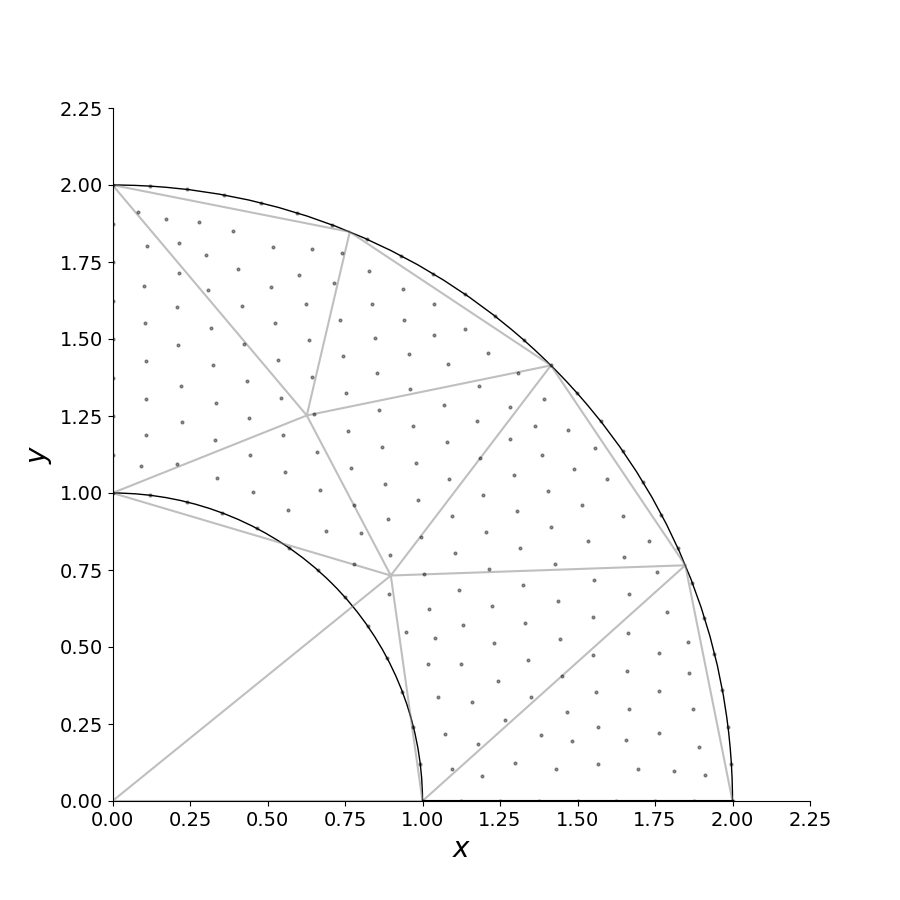
\includegraphics[scale=0.6]{../results/thick_walled_cylinder/pressure_only/core/area_coarse_simplified_cylinder.png}}
\caption{Схема грубой расчётной области для третьей тестовой задачи}
\label{fig:task_03_area_coarse_1}
\end{figure}

\newpage

В таблице \ref{table:task_03_add2_iters} представлено количество итераций в зависимости от количества подобластей и шага сетки при использовании двухуровневого аддитивного метода Шварца в случае фиксированного относительного перекрытия подобластей (данный коэффициент равен 0.3). Анализ полученных результатов показал, что:
\begin{itemize}
\item количество итераций не зависит от шага сетки;
\item при увеличении числа подобластей количество итераций не меняется;
\end{itemize}

\begin{table}[h]
\caption{Количество итераций в зависимости от количества подобластей и шага сетки для двухуровневого аддитивного метода Шварца}
\csvloop{
	file = ../results/thick_walled_cylinder/pressure_only/schwarz_two_level_additive/iters_simplified_cylinder.csv,
	head to column names,
	before reading = \centering\sisetup{table-number-alignment=center},
	tabular = {
		@{} |
		c |
		c | 
		c |
		c |
		@{}
	},
	table head = \hline Количество подобластей & \text{h = 0.05} & \text{h = 0.025} & \text{h = 0.0125} \\\hline,
	command = \amnt & \first & \second & \third,
	late after line = \\\hline
}
\label{table:task_03_add2_iters_coarse_1}
\end{table}

В таблице \ref{table:task_03_iters_overlap} рассмотрена зависимость количества итераций для различных вариантов методов декомпозиции области от коэффициента относительного перекрытия для случая 4 подобластей и шага сетки $h = 0.025$. Анализ полученных результатов показал, что:
\begin{itemize}
\item при росте коэффициента относительного захлёста количество итераций уменьшается
\end{itemize}

\begin{table}[h]
\caption{Количество итераций в зависимости от метода декомпозиции области и коэффициента относительного захлёста для случая $M = 4$ и $h = 0.025$}
\csvloop{
	file = ../results/thick_walled_cylinder/pressure_only/core/overlap_simplified_cylinder.csv,
	head to column names,
	before reading = \centering\sisetup{table-number-alignment=center},
	tabular = {
		@{} |
		c |
		c |
		c |
		c |
		@{}
	},
	table head = \hline Коэффициент относительного захлёста & 0.2 & 0.3 & 0.4 \\\hline,
	command = \method & \0 & \1 & \2,
	late after line = \\\hline
}
\label{table:task_03_iters_overlap_coarse_1}
\end{table}

\newpage

\subsection{Четвёртая тестовая задача}

На рис. \ref{fig:task_04_scheme} представлена расчётная область для четвёртой тестовой задачи - сектор поперечного сечения модели подшипника, нагруженной внешним давлением $p = 5$ МПа. Внутренний радиус $p_a = 1$ см, внешний радиус $p_b = 2 $ см.

\begin{figure}[h]
\center{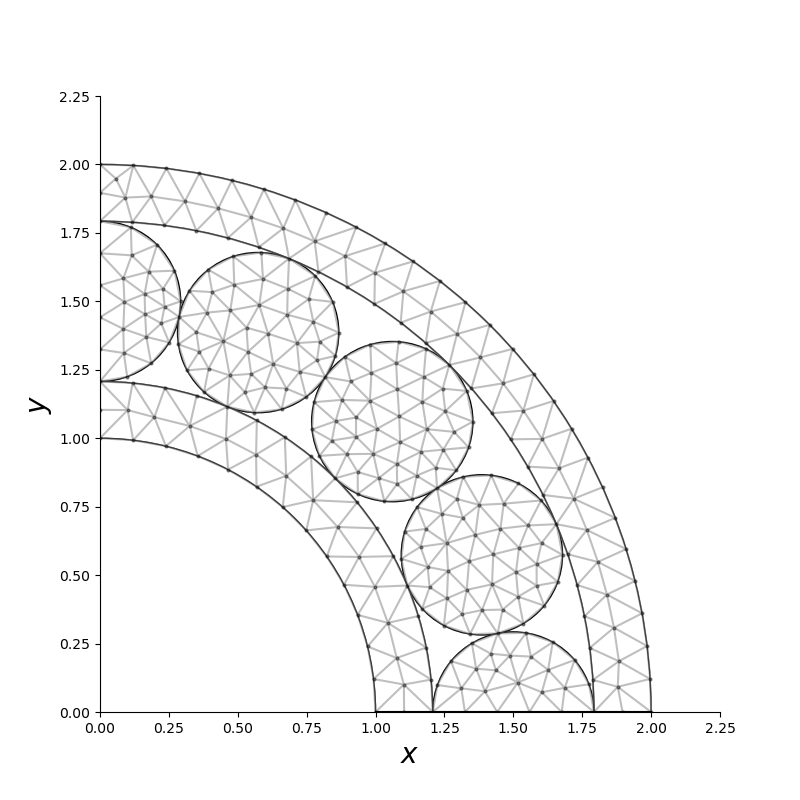
\includegraphics[scale=0.9]{../results/bearing/pressure_only/core/area_diagram.png}}
\caption{Схема расчётной области третьей тестовой задачи}
\label{fig:task_04_scheme}
\end{figure}

Для решения поставленной задачи примем, что материал тела имеет следующие параметры: модуль Юнга $E = 70$ ГПа, коэффициент Пуассона $\mu = 0.34$. 

Для исследования зависимости сходимости метода от размерности итоговой системы линейных уравнений рассмотрены три расчётные сетки с шагами $h = 0.05$ (количество узлов - 994), $h = 0.025$ (количество узлов - 3812), $h = 0.0125$ (количество узлов - 15006).

Для аддитивного метода Шварца итерационный параметр $\alpha = 0.5$.

\newpage

Для решения задачи методами декомпозиции области расчётная область разбивается на заданное количество секторов без перекрытия $\Omega_1, \ldots, \Omega_M$. 

Характерные размеры каждой подобласти: угол каждого сектора-подобласти $\varphi_M = \pi / (2 \cdot M)$. На рис. \ref{fig:task_04_decomposition} представлена расчётная область третьей тестовой задачи, разбитая на две подобласти.

\begin{figure}[h]
\center{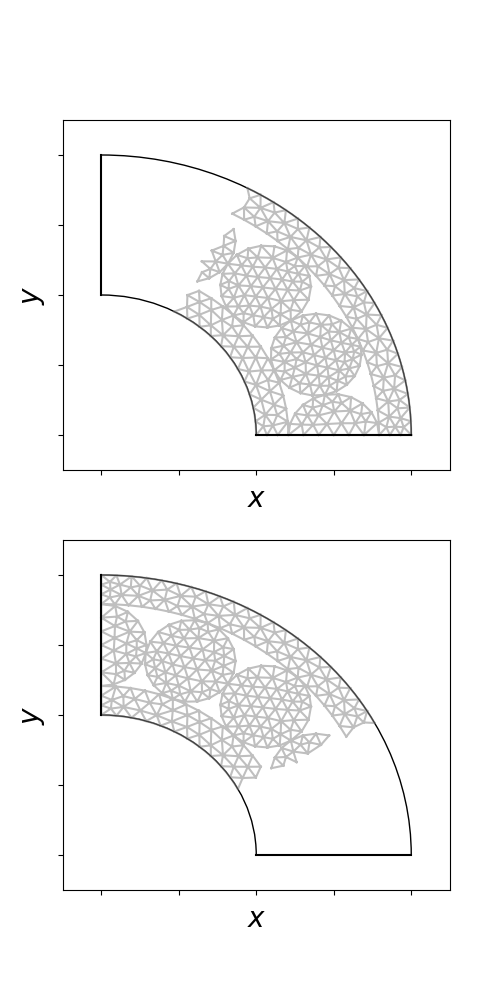
\includegraphics[scale=0.75]{../results/bearing/pressure_only/core/area_decomposition.png}}
\caption{Схема декомпозиции расчётной области третьей тестовой задачи}
\label{fig:task_04_decomposition}
\end{figure}

\newpage

Для четвёртой тестовой задачи известно аналитическое решение для компонент вектора перемещений и тензора напряжений. На рис. \ref{fig:task_04_basic_displacement_distribution} приведено распределение перемещений, полученных при решении задачи без методов декомпозиции области, на рис. \ref{fig:task_04_basic_pressure_distribution} - распределение напряжений вблизи области приложения давления.

\begin{figure}[h]
\center{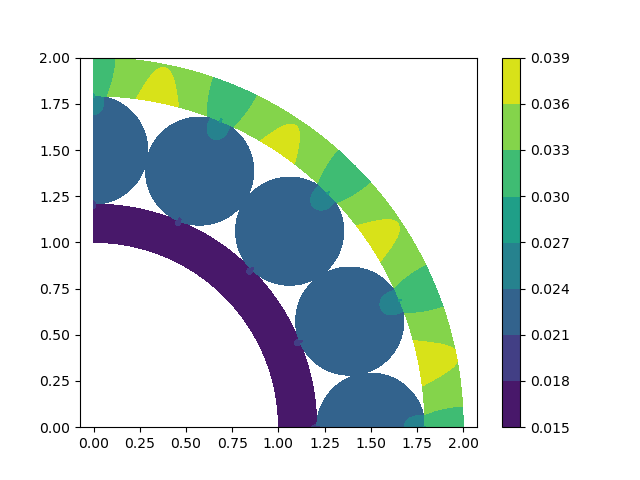
\includegraphics[scale=0.7]{../results/bearing/pressure_only/basic_method/displacement_distribution.png}}
\caption{Распределение перемещений во всей расчётной области}
\label{fig:task_04_basic_displacement_distribution}
\end{figure}

\begin{figure}[h]
\center{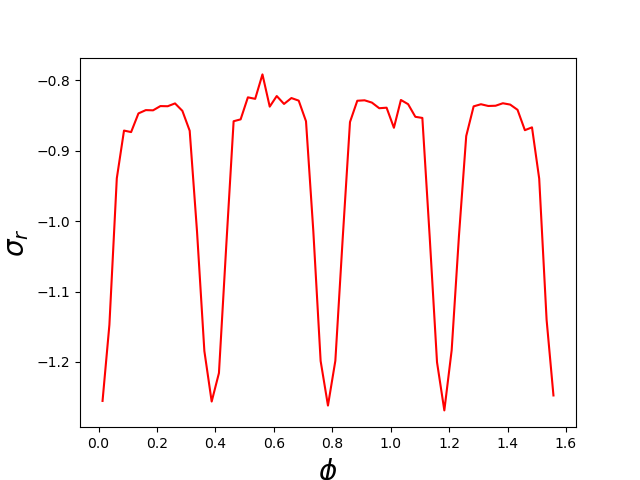
\includegraphics[scale=0.65]{../results/bearing/pressure_only/basic_method/pressure_distribution.png}}
\caption{Распределение напряжений вблизи области приложения давления}
\label{fig:task_04_basic_pressure_distribution}
\end{figure}

\newpage

\subsubsection{Мультипликативный метод Шварца}

В таблице \ref{table:task_04_mult_iters} представлено количество итераций в зависимости от количества подобластей и шага сетки при использовании мультипликативного метода Шварца для второй тестовой задачи (коэффициент захлёста для подобластей равен 0.3). Анализ полученных результатов показал, что:
\begin{itemize}
\item количество итераций не зависит от шага сетки;
\item при увеличении числа подобластей количество итераций увеличивается;
\end{itemize}

\begin{table}[h]
\caption{Количество итераций в зависимости от количества подобластей и шага сетки для мультипликативного метода Шварца}
\csvloop{
	file = ../results/bearing/pressure_only/schwarz_multiplicative/iters_bearing.csv,
	head to column names,
	before reading = \centering\sisetup{table-number-alignment=center},
	tabular = {
		@{} |
		c |
		c | 
		c |
		c |
		@{}
	},
	table head = \hline Количество подобластей & \text{h = 0.05} & \text{h = 0.025} & \text{h = 0.0125} \\\hline,
	command = \amnt & \first & \second & \third,
	late after line = \\\hline
}
\label{table:task_04_mult_iters}
\end{table}

\subsubsection{Аддитивный метод Шварца}

В таблице \ref{table:task_04_add_iters} представлено количество итераций в зависимости от количества подобластей и шага сетки при использовании аддитивного метода Шварца для второй тестовой задачи (коэффициент захлёста для подобластей равен 0.3). Анализ полученных результатов показал, что:
\begin{itemize}
\item количество итераций не зависит от шага сетки;
\item при увеличении числа подобластей количество итераций увеличивается;
\end{itemize}

\begin{table}[h]
\caption{Количество итераций в зависимости от количества подобластей и шага сетки для аддитивного метода Шварца}
\csvloop{
	file = ../results/bearing/pressure_only/schwarz_additive/iters_bearing.csv,
	head to column names,
	before reading = \centering\sisetup{table-number-alignment=center},
	tabular = {
		@{} |
		c |
		c | 
		c |
		c |
		@{}
	},
	table head = \hline Количество подобластей & \text{h = 0.05} & \text{h = 0.025} & \text{h = 0.0125} \\\hline,
	command = \amnt & \first & \second & \third,
	late after line = \\\hline
}
\label{table:task_04_add_iters}
\end{table}

\newpage

\subsubsection{Двухуровневый аддитивный метод Шварца}

В таблице \ref{table:task_04_add2_iters} представлено количество итераций в зависимости от количества подобластей и шага сетки при использовании двухуровневого аддитивного метода Шварца для первой тестовой задачи (коэффициент захлёста для подобластей равен 0.3). Анализ полученных результатов показал, что:
\begin{itemize}
\item количество итераций не зависит от шага сетки;
\item при увеличении числа подобластей количество итераций не меняется;
\end{itemize}

\begin{table}[h]
\caption{Количество итераций в зависимости от количества подобластей и шага сетки для двухуровневого аддитивного метода Шварца}
\csvloop{
	file = ../results/bearing/pressure_only/schwarz_two_level_additive/iters_thick_walled_cylinder.csv,
	head to column names,
	before reading = \centering\sisetup{table-number-alignment=center},
	tabular = {
		@{} |
		c |
		c | 
		c |
		c |
		@{}
	},
	table head = \hline Количество подобластей & \text{h = 0.05} & \text{h = 0.025} & \text{h = 0.0125} \\\hline,
	command = \amnt & \first & \second & \third,
	late after line = \\\hline
}
\label{table:task_04_add2_iters}
\end{table}

В таблице \ref{table:task_04_iters_overlap} рассмотрена зависимость количества итераций для различных вариантов методов декомпозиции области от коэффициента относительного перекрытия для случая 4 подобластей и шага сетки $h = 0.025$. Анализ полученных результатов показал, что:
\begin{itemize}
\item при росте коэффициента относительного захлёста количество итераций уменьшается
\end{itemize}

\begin{table}[h]
\caption{Количество итераций в зависимости от метода декомпозиции области и коэффициента относительного захлёста для случая $M = 4$ и $h = 0.025$}
\csvloop{
	file = ../results/bearing/pressure_only/core/overlap_thick_walled_cylinder.csv,
	head to column names,
	before reading = \centering\sisetup{table-number-alignment=center},
	tabular = {
		@{} |
		c |
		c |
		c |
		c |
		@{}
	},
	table head = \hline Коэффициент относительного захлёста & 0.2 & 0.3 & 0.4 \\\hline,
	command = \method & \0 & \1 & \2,
	late after line = \\\hline
}
\label{table:task_04_iters_overlap}
\end{table}

\newpage

Для улучшения ситуации решения третьей тестовой задачи двухуровневым аддитивным методом можно использовать в качестве грубой сетки сектор поперечного сечения цилиндра. Радиус цилиндра совпадает с внешним радиусом толстостенной трубы.

\begin{figure}[h]
\center{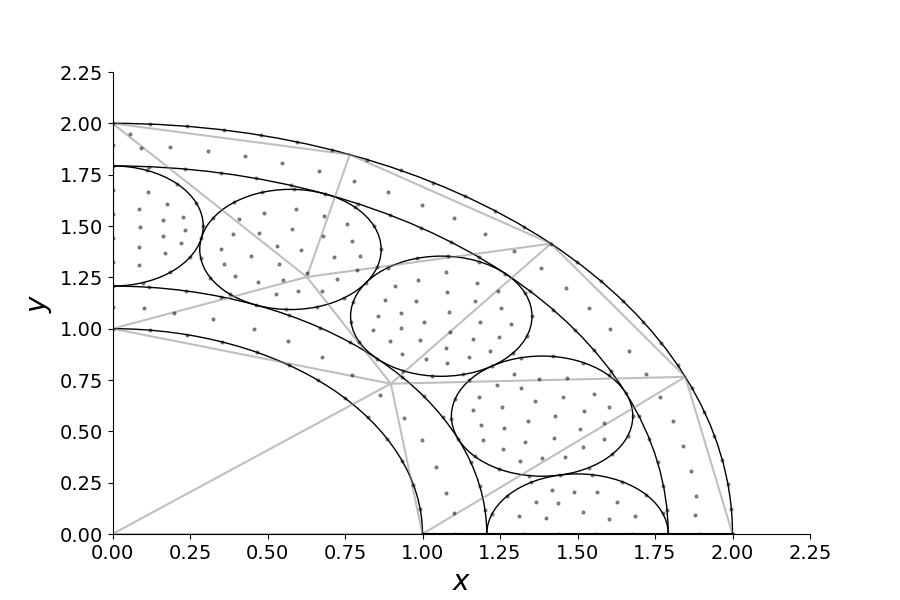
\includegraphics[scale=0.6]{../results/bearing/pressure_only/core/area_coarse_simplified_cylinder.png}}
\caption{Схема грубой расчётной области для третьей тестовой задачи}
\label{fig:task_04_area_coarse_1}
\end{figure}

\newpage

В таблице \ref{table:task_04_add2_iters} представлено количество итераций в зависимости от количества подобластей и шага сетки при использовании двухуровневого аддитивного метода Шварца в случае фиксированного относительного перекрытия подобластей (данный коэффициент равен 0.3). Анализ полученных результатов показал, что:
\begin{itemize}
\item количество итераций не зависит от шага сетки;
\item при увеличении числа подобластей количество итераций не меняется;
\end{itemize}

\begin{table}[h]
\caption{Количество итераций в зависимости от количества подобластей и шага сетки для двухуровневого аддитивного метода Шварца}
\csvloop{
	file = ../results/bearing/pressure_only/schwarz_two_level_additive/iters_simplified_cylinder.csv,
	head to column names,
	before reading = \centering\sisetup{table-number-alignment=center},
	tabular = {
		@{} |
		c |
		c | 
		c |
		c |
		@{}
	},
	table head = \hline Количество подобластей & \text{h = 0.05} & \text{h = 0.025} & \text{h = 0.0125} \\\hline,
	command = \amnt & \first & \second & \third,
	late after line = \\\hline
}
\label{table:task_04_add2_iters_coarse_1}
\end{table}

В таблице \ref{table:task_04_iters_overlap} рассмотрена зависимость количества итераций для различных вариантов методов декомпозиции области от коэффициента относительного перекрытия для случая 4 подобластей и шага сетки $h = 0.025$. Анализ полученных результатов показал, что:
\begin{itemize}
\item при росте коэффициента относительного захлёста количество итераций уменьшается
\end{itemize}

\begin{table}[h]
\caption{Количество итераций в зависимости от метода декомпозиции области и коэффициента относительного захлёста для случая $M = 4$ и $h = 0.025$}
\csvloop{
	file = ../results/bearing/pressure_only/core/overlap_simplified_cylinder.csv,
	head to column names,
	before reading = \centering\sisetup{table-number-alignment=center},
	tabular = {
		@{} |
		c |
		c |
		c |
		c |
		@{}
	},
	table head = \hline Коэффициент относительного захлёста & 0.2 & 0.3 & 0.4 \\\hline,
	command = \method & \0 & \1 & \2,
	late after line = \\\hline
}
\label{table:task_04_iters_overlap_coarse_1}
\end{table}

\end{document}
